\documentclass[review]{elsarticle}

\usepackage{lineno,hyperref}
\usepackage{listings}
\usepackage{color}
\usepackage{url}
\modulolinenumbers[5]

\journal{Journal of Parallel and Distributed Computing}

%%%%%%%%%%%%%%%%%%%%%%%
%% Elsevier bibliography styles
%%%%%%%%%%%%%%%%%%%%%%%
%% To change the style, put a % in front of the second line of the current style and
%% remove the % from the second line of the style you would like to use.
%%%%%%%%%%%%%%%%%%%%%%%

%% Numbered
%\bibliographystyle{model1-num-names}

%% Numbered without titles
%\bibliographystyle{model1a-num-names}

%% Harvard
%\bibliographystyle{model2-names.bst}\biboptions{authoryear}

%% Vancouver numbered
%\usepackage{numcompress}\bibliographystyle{model3-num-names}

%% Vancouver name/year
%\usepackage{numcompress}\bibliographystyle{model4-names}\biboptions{authoryear}

%% APA style
%\bibliographystyle{model5-names}\biboptions{authoryear}

%% AMA style
%\usepackage{numcompress}\bibliographystyle{model6-num-names}

%% `Elsevier LaTeX' style
\bibliographystyle{elsarticle-num}
%%%%%%%%%%%%%%%%%%%%%%%

\begin{document}

\begin{frontmatter}

\title{BOAST: a Metaprogramming Framework to Produce Portable and Efficient Computing Kernels for HPC Applications}

%% or include affiliations in footnotes:
\author[mymainaddress]{Brice Videau}
\ead{brice.videau@imag.fr}
\author{Kevin Pouget}
\author{Luigi Genovese}
\author{Thierry Deutsch}
\author{Dimitri Komatitsch}
\author{Jean-François Méhaut}

\address[mymainaddress]{LIG/CNRS}

\begin{abstract}
The Abstract.
\end{abstract}

\begin{keyword}
Code Generation \sep Portability \sep Genericity \sep Productivity and Software
Design \sep High Performance Computing \sep Autotuning \sep Non Regression
Testing
\end{keyword}

\end{frontmatter}

\linenumbers

\section{Introduction}

Porting and tuning HPC applications to new platforms is tedious and costly in
term of human resources.

Portability efforts are often lost when migrating to a new architecture, or code
lose maintainability because several versions of the code coexist, usually with
a lot of duplication.

Thus productivity of porting and tuning efforts is low as a huge fraction of
those developments are never used after the platform they were intended for is
decommissioned.

Genericity of HPC codes is often limited. Producing generic code in FORTRAN
90/95 is difficult as the language is not really  fit for it.

Functionality of HPC codes is tied to the previous point. Without genericity,
adding new functionalities can be quite costly.

\section{Background and Motivation}



  \subsection{Evolution of HPC Architectures}

Evolution of HPC Architectures is rapid and also diverse: in the last 5
years no less than 6 architectures have been number one in the Top500:
\begin{itemize}
\item Intel Processor + Xeon Phi (Tianhe-2)
\item AMD Processor + NVIDIA GPU (Titan)
\item IBM BlueGene/Q (Sequoia)
\item Fujitsu SPARC64 (K computer)
\item Intel Processor + NVIDIA GPU (Tianhe-1)
\item AMD Processor (Jaguar)
\end{itemize}
Being able to efficiently use those architectures on such a small
time-frame is challenging. Stress frequency of architecture changes.

The race to exascale is not going to simplify the environment. All of the above
architectures can be considered. Network architectures are also part of the
architecture and can be very diverse.  For instance European FP7 project DEEP
considers using Accelerators (XEON Phi) while the European FP7 project
Mont-Blanc considers using low-power embedded processor with integrated GPU.

Running existing applications on those new architectures is an open project.
Thus, those projects have work packages dedicated to applications. Those
workpackages are dedicated to porting and optimizing Scientific applications on
those new architectures. In the DEEP project six applications were selected for
porting and optimizing, eleven were selected in the Mont-Blanc project.
 
  \subsection{Scientific Computing Applications}

Developed by physicist, chemist, meteorologist. Usually in FORTRAN for
historical and performance reason. Codes can be quite huge (several
thousands lines of code) with lots of functionalities. Nonetheless they are
usually based on computing kernels. Computing kernels are resource
intensive and well defined parts of a program with a limited set of input
and output. Those kernels are the time consuming part of an HPC
application. They are thus the prime target for optimization.

Those applications are often developed by several individuals. Sometimes some of
those developers only work a few month on the application. Maintaining optimized
code written by someone else is quite a challenge.

In Section~\ref{use_cases} we will present two HPC application that we used
as use cases: SPECFEM3D and BigDFT. They are both based on computing
kernels and were selected as candidate applications in the Mont-Blanc project.

  \subsection{How Should Computing Kernels be Written?}

The problematic here is to obtain computing kernels that present good
performances on the architectures encountered by the application while still
being portable after the optimization process took place. Indeed the application
might encounter one of the other architectures presented before. Investing
manpower to optimize the application for a new architecture is reasonable,
suffering hindrance from previous optimization work is not. Thus optimizations
have to be as orthogonal as possible from one another so as to be easily
activated and deactivated.

If this paradigm is followed by developers then they will rapidly be confronted
with a huge optimization space to search. They will need to be able to test
easily the performance impact of the chosen optimizations without running the
full application. The same reasoning implies that kernels should be tested for
non regression without running the full application.

What we want is computing kernels that are:
\begin{itemize}
\item Written in a \emph{portable} manner,
\item Written in a way that raise developer \emph{productivity},
\item Written to present good \emph{performance}.
\end{itemize}

\section{BOAST: Using Code Generation in Application Autotuning}

  Provide scientific application developers with a framework to develop and test
application computing kernels. Two aspects should be considered:
\begin{itemize}
\item code description,
\item code generation and kernel execution runtime.
\end{itemize}

\begin{center}
\begin{figure}
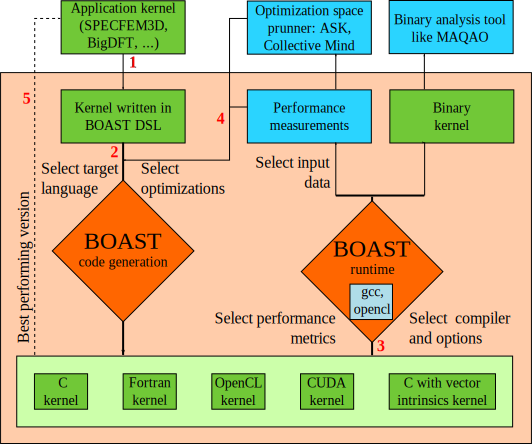
\includegraphics[width=\textwidth]{BOAST_Workflow.pdf}
\caption{Structure and Workflow of the BOAST framework.}
\label{fig:boast_workflow}
\end{figure}
\end{center}

  \cite{videau2013boast}

  \subsection{Kernel Description Language}

  \begin{itemize}
  \item Abstraction of programming concepts: variables, procedures (
portability, productivity )
  \item Operator overloading: simpler syntax ( productivity, portability )
  \item Two languages in one ( productivity, performance ) 
  \end{itemize}

Usually computing kernels are hotspots of an HPC application, and are most of
the time based on a loop nest. A lot of effort is dedicated to their tuning and
the obtained result is often quite different than the original procedure.
Several transformations can be applied to such kernels. And those optimization
are often applied manually as compiler may fail to recognise the opportunity.

There are many different loop optimization techniques~\cite{wolf1991loop}. We
can cite loop skewing~\cite{wolfe1986loops} (derives nested loops wavefronts)
or loop interchange~\cite{allen1984automatic} (loop variables change places).

The importance of  correct loop imbrication on BLAS~\cite{lawson1979basic}
operations is studied in~\cite{soliman2009performance}, and shows performance
increase of a factor up to 5 when using correct loop imbrication. The importance
of code transformation is stressed in~\cite{ye2011porting}, where a selection of GPU
kernels are ported to CPU and optimized.

BOAST kernel description language should be able to express all these
optimizations. This gives us a set of constraints to implement in the language:
\begin{itemize}
\item Arbitrary number of variables have to be created and manipulated (types,
attributes...).
\item Procedures have to be abstracted (reunite FORTRAN and C like languages,
attributes...).
\item Functions must be available.
\item Variables, constants and functions must be composed in complex
Expressions.
\item Basic control structures (for, while, if/else...) have to be abstracted.
\item Powerful array management (several dimensions, transformations,
indexing...).
\end{itemize}

In order to manipulate those abstractions we want to have a syntax resembling
what programmers use. For instance commonly used operator have to be available
and behave as expected. It must also be possible to differentiate an action on
an abstraction in the context of an expression and in the context of the
management of this expression. This is why an embedded domain specific language
approach was selected~\cite{hudak1996building}. This allows for the coexistence
of two languages: the host language and the DSL. In our case the DSL allows the
description of the kernel while the host language provides the meta programming
of the kernel. Operator overloading of the host language will provide the
familiar syntax programmers are accustomed to.

It was also important to have our constructs like \emph{for loops} to have a
syntax approaching those commonly found in programming languages. For this we
needed a language which could seamlessly pass a block of code to a function.
Ruby~\cite{matsumoto2002ruby} is one such language. It has deep introspection
capabilities as well.

    \subsubsection{BOAST keywords}

  In order to clearly differentiate what is going to be generated from what is
related to manipulations in the host language the \emph{print} method was
redefined in the BOAST namespace. This print method only insures that the object
it is called on implements a public print method. Each BOAST object is
responsible for printing itself correctly depending on the BOAST configuration
at the time the print public method is called.

  

    \subsubsection{BOAST Abstractions}

  Variable

  Expression

  If

  For

  While

  Case
  
%Considering source-to-source transformations that we investigate with the BOAST
%tool in this paper, we can compare ourselves to POET~\cite{POET2012}  and
%ABCLibScript~\cite{ABCLib2006}. However, both tools apply transformations
%to the syntaxic tree of a program while BOAST intervenes well before in the
%transformation process. Indeed, one may first use BOAST on order to generate a
%program (a specific syntaxic tree) and then benefit from the transformation
%facilities offered by one of the above tools.

  \subsection{BOAST Runtime}

  \begin{itemize}
  \item multi target language generation ( performance, portability )
  \item compilation ( productivity, performance )
  \item execution ( productivity, performance )
  \item tracer, dumper and replay for non regression tests ( productivity )
  \end{itemize}

\section{Use Cases}
\label{use_cases}

  \subsection{Creating an Auto-Tuned Convolution Library for BigDFT using BOAST}

    \subsubsection{BigDFT}

BigDFT~\cite{bigdft} is a scientific application computing the electronic
structure of systems using density functional
theory (DFT). The application is mainly written in Fortran and currently
includes some 193,000 lines of Fortran code, which accounts for more than 50 \% 
of the code base. It is a parallel application based on the standards
MPI~\cite{mpi} and OpenMP~\cite{openmp}.  It also supports CUDA~\cite{cuda} and
OpenCL~\cite{opencl}.  As it is used on systems that may
have very different architectures, it is of great importance to be able to
optimize and run the application according to the specific underlying platform.


BigDFT is characterized by its extensive use of
convolution operators~\cite{nussbaumer1982fast} applied on large arrays of
data.  One example of a specific convolution, called
MagicFilter~\cite{Genovese|CAS2010}, can be seen in Listing~\ref{lst:conv_example}. 
It applies a filter $filt$ to the data set $in$ and then stores the result in the data set $out$ with a
transposition~\cite{Goedecker1993}.

\lstset{	language=C, 
		basicstyle=\scriptsize, 
		backgroundcolor=\color{white}, 
		frame=single, 
		captionpos=b,
		caption={MagicFilter}, 
		label={lst:conv_example}}
		
\begin{lstlisting}
double filt[16] = {F0, F1, ... , F15};
void magicfilter(int n, int ndat, double* in, double* out){
  double temp;
  int m;
  for( j = 0; j < ndat; j++) {
    for( i = 0; i < n; i++) {
      temp = 0;
      for( k = 0; k < 16; k++) {
        m = (i-7+k)%n
        temp += in[m + j*n] * filt[k];
      }
      out [j + i*ndat] = temp ;
    } 
  }
} 
\end{lstlisting}

As we can see, there are three nested loops working on arrays whose sizes
vary.  Various optimizations can be applied to this treatment and
may focus on the loop structure, as well as on the size of the data.  In this
paper we focus on this particular convolution and explore different
optimizations whose nature is presented in detail in the next section.

    \subsubsection{A Generic Convolution Library}

  BigDFT implementation of convolution/wavelets is a reference but is limited in scope (1 wavelet family ands its derived operators).
  Generalizing to other wavelet families long and difficult if performance are to remain good.

Idea:
\begin{itemize}
\item write a generic convolution library in BOAST
\item BLAS like interface
\item Provide a wide variety of building blocks
\item Optimize thos blocks using BOAST
\item Build either from source or directly link with binary
\item Release complete library
\end{itemize}


  Characteristic use case driven

  Convolution Library: first step toward a dsl dedicated to wavelet processing for Physics computing.

  \subsection{Porting SPECFEM3D to OpenCL using BOAST}

    \subsubsection{SPECFEM3D}

\begin{itemize}

\item Wave propagation research software

\item HPC application (benchmark on supercomputers)

\item Complex GPU (CUDA) code, 40+ kernels.

\item 80+ parameters for kernels. Difficult to validate.
\end{itemize}

    \subsubsection{Porting to OpenCL}

  Idea:
\begin{itemize}
\item write kernels in BOAST,
\item generate kernels in CUDA,
\item validate kernels by comparing CUDA/generated CUDA executions using comparator
\item generate kernels in OpenCL,
\item develop OpenCL runtime backend using previously validated OpenCL kernels
\item validate OpenCL version by comparing CUDA/OpenCL executions using comparator
\end{itemize}

  Evaluation:
\begin{itemize}
\item Similar CUDA/OpenCL
\item Factoring : more compact code
\item Integrated non regression support
\item Integrated Kernel performance evaluation
\end{itemize}

\section{Related Work}

  \subsection{Kernel Description DSL}

  Orio

  Halide

  Spiral

  POET

  \subsection{Application Autotuning}

  Atlas

  Orio

  Halide

  \subsection{Optimization Space Pruner}

  Collective Mind

  Adaptive Sampling Kit (ASK)

\section{Conclusion and Future Works}


\section*{References}

\bibliography{BOAST}

\end{document}
